\paragraph{}En este proceso, el usuario asesor puede crear, consultar, modificar
o borrar plantillas de asesor de la aplicación.

\paragraph{}La figura \ref{diagramaNivel4-AdministrarPlantillasAsesor}
muestra el nivel de abstracción 4: Administrar plantillas de asesor.

  \begin{figure}[!ht]
    \begin{center}
      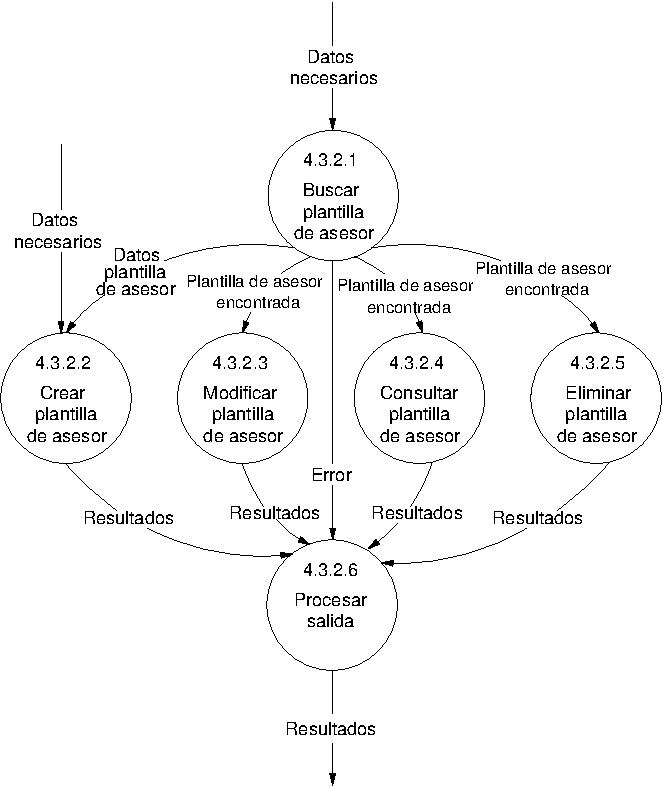
\includegraphics[]{08.Analisis_Funcional/8.2.DFDs/Niveles/Nivel4/Asesor/AdministrarPlantillasAsesor/Diagramas/nivel4-AdministrarPlantillasAsesor.pdf}
      \caption{Nivel de abstracción 4: Administrar plantillas de asesor.}
      \label{diagramaNivel4-AdministrarPlantillasAsesor}
    \end{center}
  \end{figure}
